\documentclass[aspectratio=169]{beamer}
%[handout]

\usetheme[progressbar=frametitle]{metropolis}
\usepackage{appendixnumberbeamer}

\usepackage[utf8]{inputenc}
\usepackage[T1]{fontenc}

\usepackage[brazil]{babel}
\usepackage[outputdir=..]{minted}
\usepackage{xcolor}
\usepackage{soul} % strikethrough
\usepackage{advdate}
\usepackage{graphicx}
\graphicspath{{figs/}}
\usepackage{graphbox}

\usepackage[ampersand]{easylist}

\usepackage{multirow}
\usepackage{multicol}
\usepackage{subcaption}

\usepackage{pgf,tikz}
\usetikzlibrary{shapes,arrows,positioning}
\usetikzlibrary{circuits.logic.US}
\usetikzlibrary{matrix,calc}

\usepackage{karnaugh-map}

\usepackage{pgfpages}
\setbeameroption{hide notes} % Only slides
% \setbeameroption{show only notes} % Only notes
% \setbeameroption{show notes on second screen=right} % Both

% \graphicspath{{../figs/}}

\definecolor{bgc}{rgb}{0.95,0.9,0.95}
\definecolor{links}{HTML}{2A7F7F}
\hypersetup{colorlinks,linkcolor=,urlcolor=links}

\newminted{verilog}{fontsize=\scriptsize, 
    linenos,
    numbersep=8pt,
    bgcolor=bgc,
    tabsize=4,
    framesep=3mm} 
    %frame=lines,

\newcommand{\verilog}[1]{\verilogf{#1}{\footnotesize}}

\newcommand{\verilogf}[2]{\inputminted[fontsize=#2, 
    linenos,
    tabsize=2,
    numbersep=4pt,
    bgcolor=bgc,
    framesep=3mm]{verilog}{../codes/#1.v}
}

\newminted{nasm}{fontsize=\scriptsize, 
		   linenos,
		   numbersep=8pt,
           bgcolor=bgc,
		   framesep=3mm} 

\usepackage{booktabs}
\usepackage[scale=2]{ccicons}

\usepackage{pgfplots}
\usepgfplotslibrary{dateplot}

\usepackage{hyperref}


\usepackage{xspace}
\newcommand{\themename}{\textbf{\textsc{metropolis}}\xspace}



\usepackage{pifont}% http://ctan.org/pkg/pifont
\newcommand{\cmark}{\ding{51}}%
\newcommand{\xmark}{\ding{55}}%

% \tiny	
% \scriptsize
% \footnotesize
% \small	
% \normalsize	
% \large	
% \Large	
% \LARGE	
% \huge	
% \Huge	



\newminted{python}{fontsize=\scriptsize, 
		   linenos,
		   breaklines,
		   numbersep=8pt,
           tabsize=2,
		   framesep=3mm} 
		   
\newminted{verilog}{fontsize=\scriptsize, 
		   linenos,
		   breaklines,
		   numbersep=8pt,
           tabsize=2,
		   framesep=3mm} 
		   




\definecolor{bgc}{rgb}{0.95,0.9,0.95}
\definecolor{links}{HTML}{2A7F7F}
\hypersetup{colorlinks,linkcolor=,urlcolor=links}


% \usepackage[style=apa]{biblatex}
% \addbibresource{mm.bib}


% \author{\large Prof. Ricardo Menotti (\href{mailto:menotti@ufscar.br}{menotti@ufscar.br})}

\newcommand{\newauthor}[2]{
  \parbox{0.50\textwidth}{
    \texorpdfstring
      {
        \centering
        \small #1 \newline
        {\scriptsize{\urlstyle{same}\href{mailto:#2}{#2}\urlstyle{tt}}}
      }
      {#1} \newline
  }
}

\author{
  \newauthor{Prof. Ricardo Menotti}{menotti@ufscar.br}
\and \newauthor{Prof. Luciano de Oliveira Neris}{lneris@ufscar.br}  
%\and \newauthor{Prof. Artino Quintino da Silva Filho}{artino@ufscar.br}
% \and \newauthor{Prof. Maurício Figueiredo}{mauricio@ufscar.br}
% \and \newauthor{Prof. Edilson Kato}{kato@ufscar.br}
% \and \newauthor{Prof. Roberto Inoue}{rsinoue@ufscar.br}
}

\date{Atualizado em: \today}

\institute{\large \textbf{Departamento de Computação} \\
Centro de Ciências Exatas e de Tecnologia \\
Universidade Federal de São Carlos}

\title{Lógica Digital (1001351)}

\titlegraphic{\hfill
\includegraphics[height=1.5cm]{LogoUfscar}}



\subtitle{Exemplos de projetos} % 

\begin{document}

\begin{frame}
	\titlepage
\end{frame} 

% Uncomment if you want a summary slide
% \begin{frame}{Conteúdo}
% 	\tableofcontents
% \end{frame}

\section{Controlador de luz com 3 entradas} %%%%%%% Can be used as slide title with \insertsection command

\begin{frame}{\insertsection} % Slide with bullets
	\begin{itemize}
		\item Em uma sala grande com três portas e um interruptor em cada porta, projete um sistema capaz de acender ou apagar as luzes da sala alterando o estado de qualquer uma das chaves;
		\item Obtenha uma função $f(x_1, x_2, x_3)$ que solucione este problema.
    \end{itemize}
    \pause
    \begin{columns}
        \begin{column}{0.40\textwidth}
        \centering
            \begin{tabular}{c|ccc||c} % center, left or right 
            \hline
            \scriptsize $linha$ & $x_1$ & $x_2$ & $x_3$ & $f$ \\
            \hline
            \hline
            \scriptsize $0$ & $0$ & $0$ & $0$ & $0$ \\
             \pause
            \scriptsize $1$ & $0$ & $0$ & $1$ & $1$ \\
             \pause
            \scriptsize $2$ & $0$ & $1$ & $0$ & $1$ \\
             \pause
            \scriptsize $3$ & $0$ & $1$ & $1$ & $0$ \\
             \pause
            \scriptsize $4$ & $1$ & $0$ & $0$ & $1$ \\
             \pause
            \scriptsize $5$ & $1$ & $0$ & $1$ & $0$ \\
             \pause
            \scriptsize $6$ & $1$ & $1$ & $0$ & $0$ \\
             \pause
            \scriptsize $7$ & $1$ & $1$ & $1$ & $1$ \\
            \hline
            \end{tabular}
        \end{column}        
        \begin{column}{0.60\textwidth}
            \pause
            $f = m_1 + m_2 + m_4 + m_7$ \\
            \vspace{0.5cm}
            \pause
            $f = \overline{x}_1\overline{x}_2x_3 + \overline{x}_1x_2\overline{x}_3 + x_1\overline{x}_2\overline{x}_3 + x_1x_2x_3$ \\
            \vspace{0.5cm}
            \pause
            $f = M_0M_3M_5M_6$ \\
            \vspace{0.5cm}
            \pause
            $f = (x_1+x_2+x_3)(x_1+\overline{x}_2+\overline{x}_3)$\\ 
            \hspace{0.65cm} $(\overline{x}_1+x_2+\overline{x}_3)(\overline{x}_1+\overline{x}_2+x_3)$
        \end{column}
    \end{columns}
\end{frame}

\begin{frame}{\insertsection} \centering
\begin{tikzpicture}[circuit logic US]
    \node[anchor=south west,inner sep=0](image) at (0,0){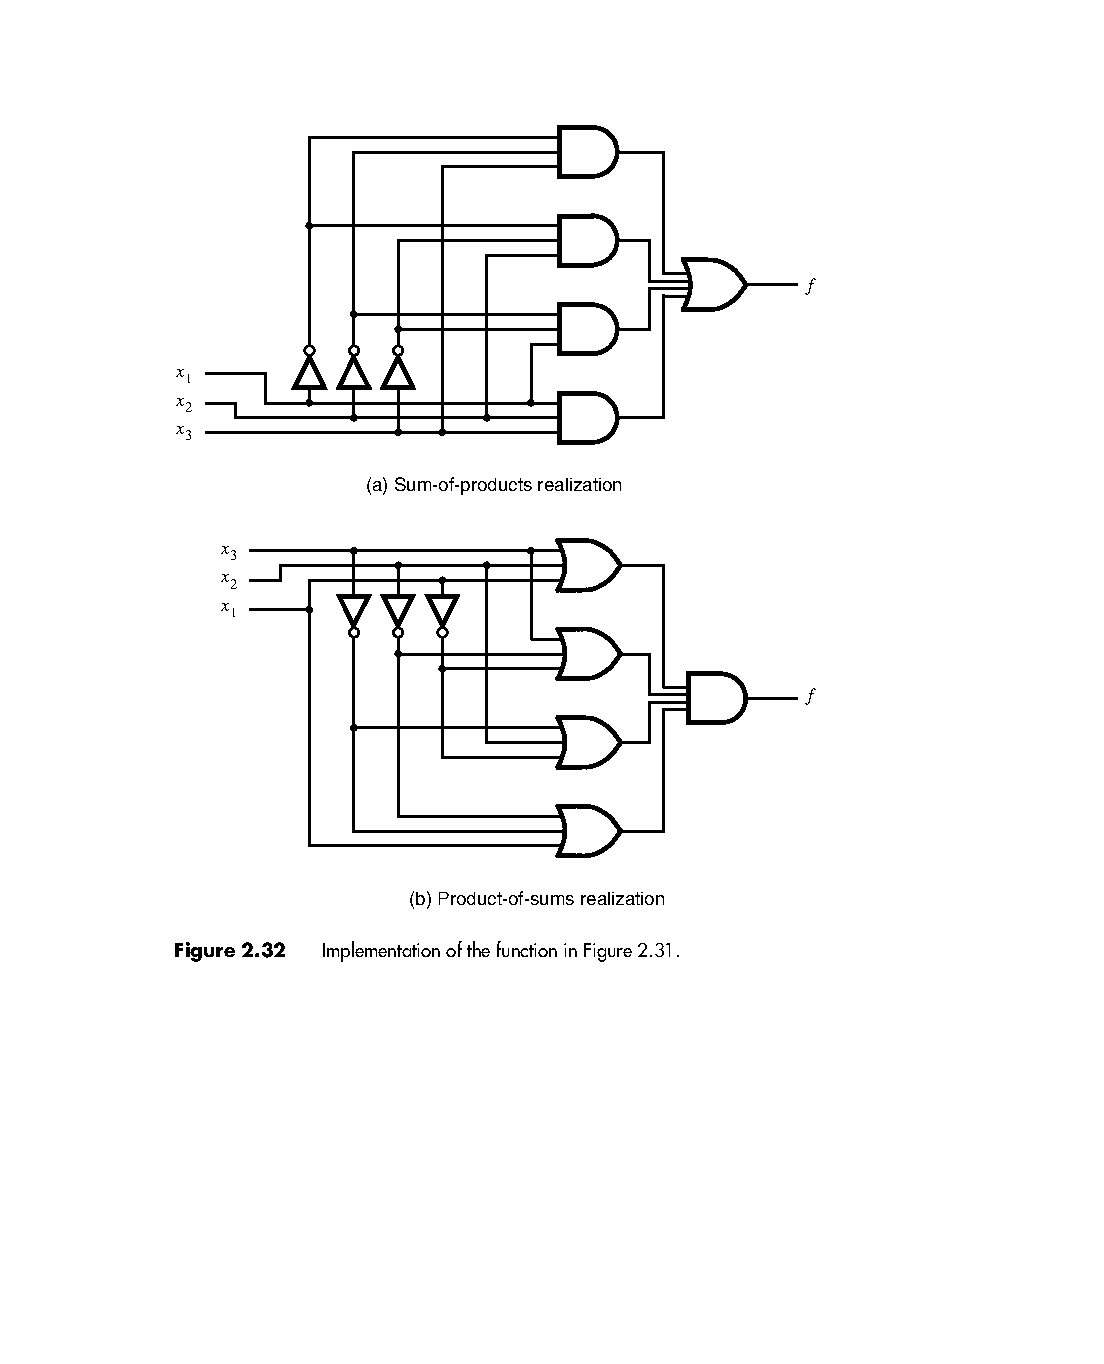
\includegraphics[width=.4\textwidth]{VerilogFig2_32}};
    \pause
    \node[xor gate, thick] (xor1) at (7, 4.5) {};   
    \draw [thick] ($(xor1.north west)!.5!(xor1.input 1)$) -- ++(left:5mm) node [left]{\footnotesize $x_1$};
    \draw [thick] ($(xor1.input 1)!.5!(xor1.input 2)$) -- ++(left:5mm) node [left]{\footnotesize $x_2$};
    \draw [thick] ($(xor1.south west)!.5!(xor1.input 2)$) -- ++(left:5mm) node [left]{\footnotesize $x_3$};
    \draw [thick] (xor1.output) -- ++(right:5mm) node [right]{\footnotesize $f$};
\end{tikzpicture}
\end{frame}


\section{Multiplexador} %%%%%%% Can be used as slide title with \insertsection command

\begin{frame}{\insertsection} % Slide with bullets
	\begin{itemize}
		\item Em sistemas de computadores, muitas vezes é necessário escolher dados de várias fontes possíveis;
		\item Suponha que haja duas fontes de dados, fornecidas como sinais de entrada $x_1$ e $x_2$; 
		\item Os valores desses sinais mudam no tempo, talvez em intervalos regulares;
		\item Queremos projetar um circuito que produza uma saída que tenha o mesmo valor de $x_1$ ou $x_2$, dependendo do valor de um sinal de controle de seleção $s$;
		\item Portanto, o circuito deve ter três entradas: $x_1$, $x_2$ e $s$;
		\item Suponha que a saída do circuito será igual ao valor da entrada $x_1$, se $s=0$, e será o valor da entrada $x_2$, se $s=1$; 
		\item Obtenha uma função $f(x_1, x_2, s)$ que solucione este problema.
    \end{itemize}
\end{frame}

\begin{frame}{\insertsection} % Slide with bullets
    \begin{columns}
        \begin{column}{0.40\textwidth}
        \centering
            \begin{tabular}{c|ccc||c} % center, left or right 
            \hline
            \scriptsize $linha$ & $s$ & $x_1$ & $x_2$ & $f$ \\
            \hline
            \hline
            \scriptsize $0$ & $0$ & $0$ & $0$ & $0$ \\
            \scriptsize $1$ & $0$ & $0$ & $1$ & $0$ \\
            \scriptsize $2$ & $0$ & $1$ & $0$ & $1$ \\
            \scriptsize $3$ & $0$ & $1$ & $1$ & $1$ \\
            \scriptsize $4$ & $1$ & $0$ & $0$ & $0$ \\
            \scriptsize $5$ & $1$ & $0$ & $1$ & $1$ \\
            \scriptsize $6$ & $1$ & $1$ & $0$ & $0$ \\
            \scriptsize $7$ & $1$ & $1$ & $1$ & $1$ \\
            \hline
            \end{tabular}
        \end{column}        
        \begin{column}{0.60\textwidth}
            \pause
            $f(s, x_1, x_2)  = \overline{s}x_1\overline{x}_2 + \overline{s}x_1x_2 + s\overline{x}_1x_2 + sx_1x_2$ \\
            \vspace{0.5cm}
            \pause
            $\overline{s}x_1(\overline{x}_2+x_2) + s(\overline{x}_1+x_1)x_2$ \\
            \vspace{0.5cm}
            \pause
            $\overline{s}x_1.1 + s.1.x_2$ \\
            \vspace{0.5cm}
            \pause
            $\overline{s}x_1 + sx_2$ \\
        \end{column}
    \end{columns}
\end{frame}

\begin{frame}{\insertsection}   \centering
    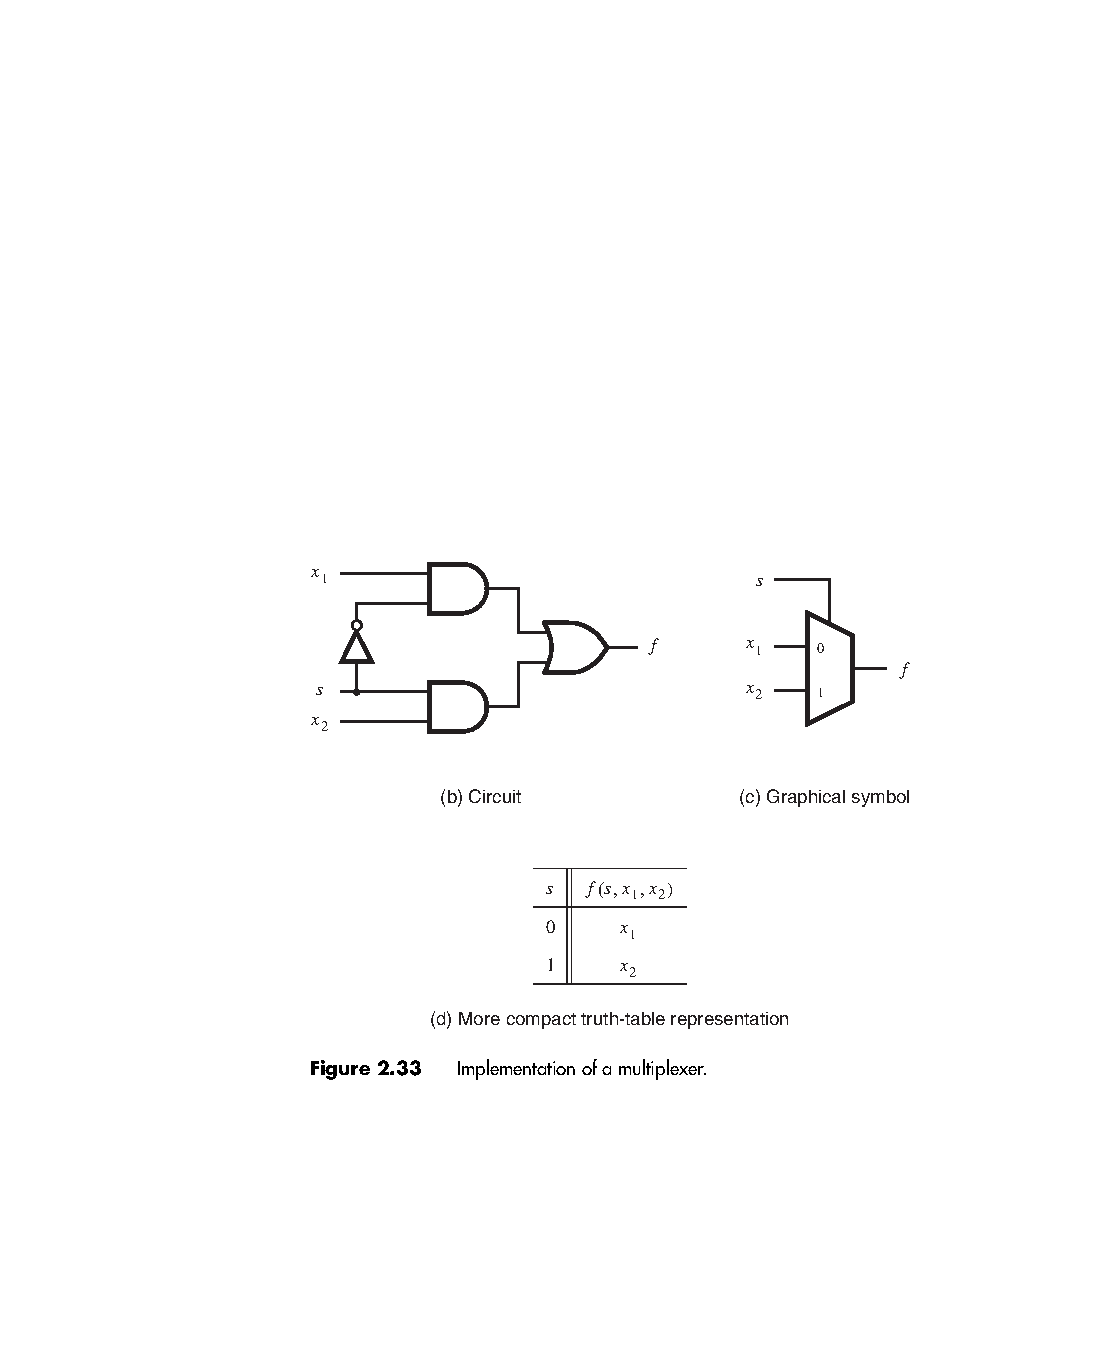
\includegraphics[width=.65\textwidth]{VerilogFig2_33}
\end{frame}

\section{Somador simplificado} %%%%%%% Can be used as slide title with \insertsection command


\begin{frame}{\insertsection}   \centering
        \begin{columns}
        \begin{column}{0.65\textwidth}
            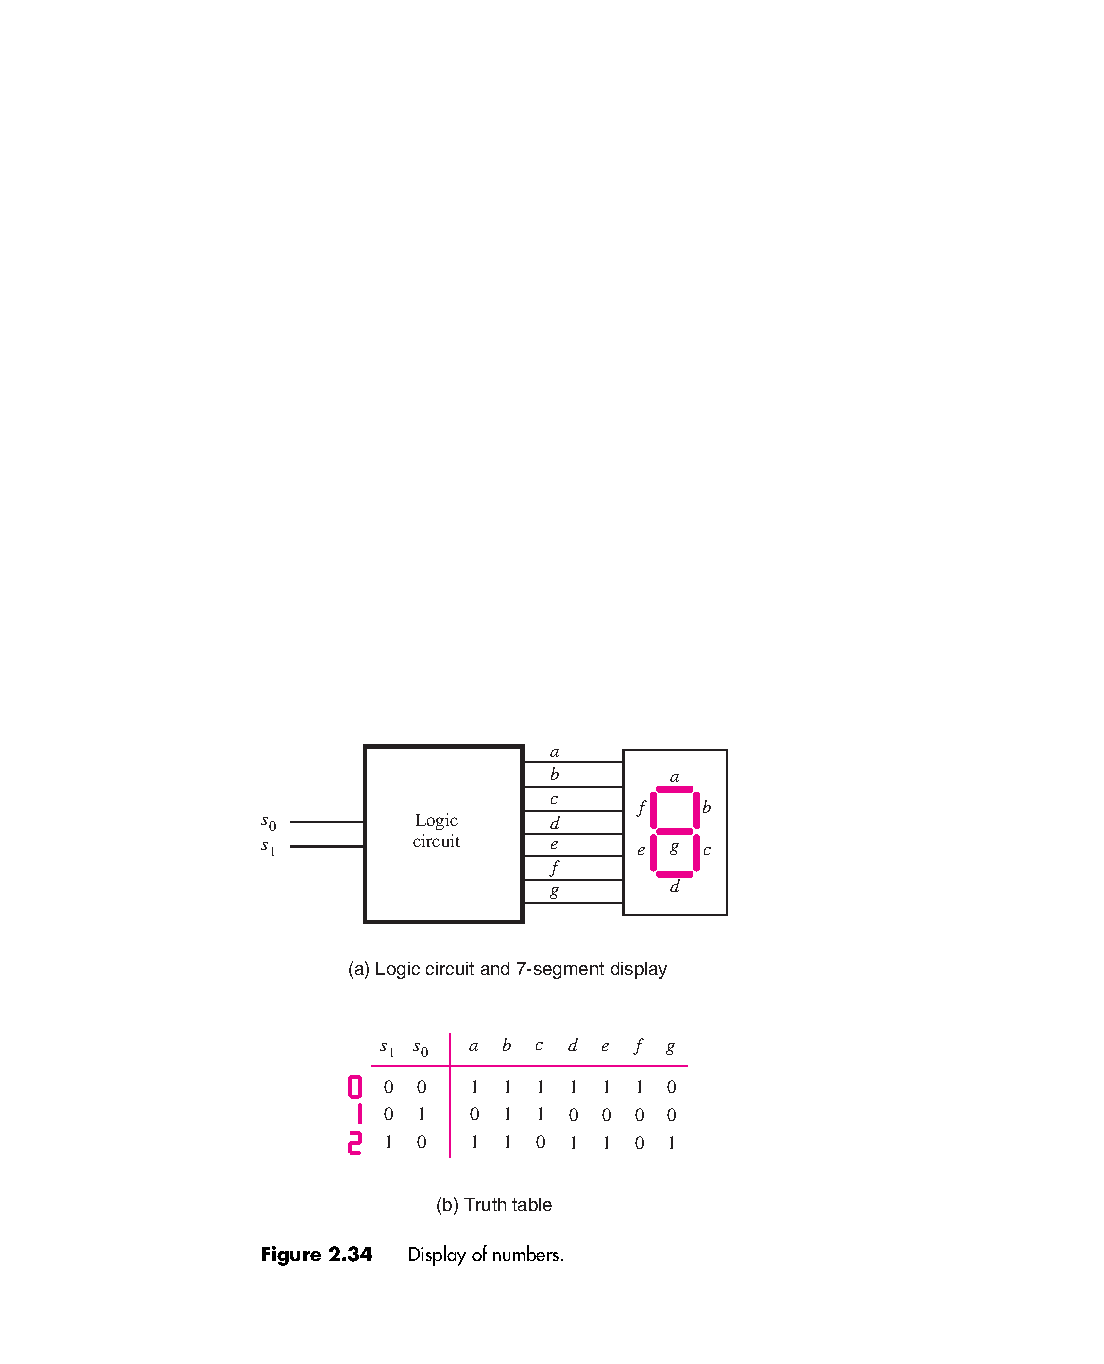
\includegraphics[width=\textwidth]{VerilogFig2_34}
        \end{column}        
        \begin{column}{0.35\textwidth}
            \pause
            $a = d = e = \overline{s}_0$ \\
            \vspace{0.5cm}
            \pause
            $b = 1$ \\
            \vspace{0.5cm}
            \pause
            $c = \overline{s}_1 $ \\
            \vspace{0.5cm}
            \pause
            $f = \overline{s}_1\overline{s}_0 $ \\
            \vspace{0.5cm}
            \pause
            $g = s_1\overline{s}_0 $ \\
        \end{column}
    \end{columns}
\end{frame}


% \section{Section table}

% \begin{frame}{\insertsection}
% 	\begin{itemize}
%         \item O intervalo de inteiros que pode ser representado por um número binário depende do número de bits usados: 
%     \end{itemize}
%     \vspace{-0.5cm} % to save space between text above and table below
%     \begin{table}[]
%         \centering \scriptsize 
%         \begin{tabular}{cc} % center, left or right 
%             \hline
%             \textbf{Decimal} & \textbf{Binária} \\
%             \hline
%             \hline
%              00 & 0000 \\
%              01 & 0001 \\
%              02 & 0010 \\
%              03 & 0011 \\
%             \hline
%         \end{tabular}
%     \end{table}
% \end{frame}

% \section{Code}

% \begin{frame}[fragile]{\insertsection}
% 	\begin{verilogcode}
% module fulladd (Cin, x, y, s, Cout); 
%   input Cin, x, y;
%   output s, Cout;

%   xor (s, x, y, Cin); 
%   and (z1, x, y);
%   and (z2, x, Cin); 
%   and (z3, y, Cin);
%   or (Cout, z1, z2, z3);
% endmodule
% 	\end{verilogcode} 
% \end{frame}

% \section{Section mixed}

% \begin{frame}{Alternative title to the section} 
%     \begin{columns}
%         \begin{column}{0.60\textwidth}
%             \begin{itemize}
%                 \item ;
%                 \item ;
%                 \item ;
%                 \item . 
%             \end{itemize}
%         \end{column}
%         \begin{column}{0.40\textwidth}
%             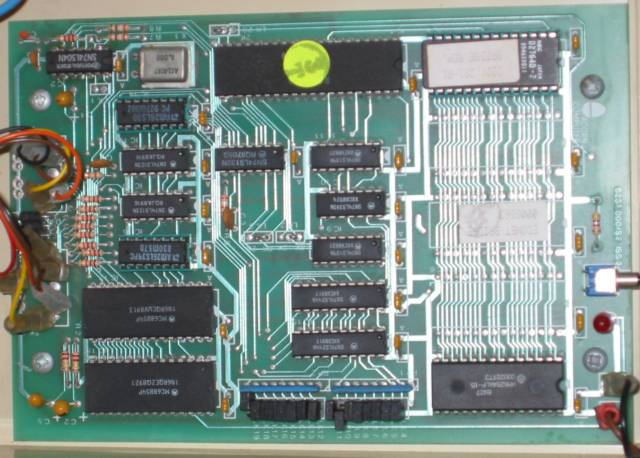
\includegraphics[angle=90,width=\textwidth]{Econet}
%         \end{column}        
%     \end{columns}
% \end{frame}

% \section{Section drawing}

% \begin{frame}{\insertsection}
%     \centering 
%     \tikzstyle{decision} = [diamond, draw, fill=red!20, text width=4.5em, text badly centered, node distance=2.3cm, inner sep=0pt]
%     \tikzstyle{block} = [rectangle, draw, fill=red!20, text width=10em, text centered, rounded corners, minimum height=2em]
%     \tikzstyle{line} = [draw, -latex']
%     \tikzstyle{cloud} = [draw, ellipse,fill=red!20, node distance=3cm,
%     minimum height=2em]
% \resizebox{0.5\textwidth}{!}{%
% \begin{tikzpicture}[node distance = 1.3cm, auto]
%     \node [cloud] (init) {Produto requerido};
%     \node [block, below of=init] (specs) {Definir espeficicação};
%     \node [block, below of=specs] (design) {Projeto inicial};
%     \node [block, below of=design] (sim) {Simulação};
%     \node [block, right=1cm of sim] (redesign) {Reprojeto};
%     \node [decision, below of=sim] (right) {Projeto correto?};
%     \node [block, below=0.7cm of right] (proto) {Prototipação};
%     \node [block, below of=proto] (test) {Testes};
%     \node [block, right=1cm of proto] (corec) {Correções};
%     \node [decision, below of=corec] (minor) {Erros menores?};
%     \node [decision, below=0.7cm of test] (meets) {Cumpre especificação?};
%     \node [cloud, below=0.3cm of meets] (finish) {Produto finalizado};
%     \path [line] (init) -- (specs);
%     \path [line] (specs) -- (design);
%     \path [line] (design) -- (sim);
%     \path [line] (sim) -- (right);
%     \path [line] (redesign) -- (sim);
%     \path [line] (right) -| (redesign) node[near start,above] {não};
%     \path [line] (right) -- (proto) node[near start,right] {sim};
%     \path [line] (proto) -- (test);
%     \path [line] (test) -- (meets);
%     \path [line] (corec) -- (proto);
%     \path [line] (minor) -- (corec) node[near start,right] {sim};
%     \path [line] (meets) -| (minor) node[near start,above] {não};
%     \path [line] (meets) -- (finish) node[near start,right] {sim};
%     \path [line] (minor.east) -- node[near start,above] {não} ++(2,0)  -- ++(0,6.95) --  (redesign.east);
% \end{tikzpicture}}
% \end{frame}

\section{Bibliografia} %%%%%%%

\begin{frame}{\insertsection} 
	\begin{itemize}
		\item \href{https://www.google.com.br/search?q=filetype\%3Apdf+Fundamentals+of+Digital+Logic+with+Verilog+Design+&oq=filetype\%3Apdf}{Brown, S. \& Vranesic, Z. - Fundamentals of Digital Logic with Verilog Design, 3rd Ed., Mc Graw Hill, 2009}
	\end{itemize}
\end{frame}

% \begin{frame}[allowframebreaks]{\insertsection} 
% 	\begin{itemize}
% 		\item Básica
% 		\begin{itemize}
% 			\item Patterson, D. A. \& Hennessy, J. L. - Organização e Projeto de Computadores - A Interface Hardware/Software 4ª Ed., Editora Campus, 2014 (14 exemplares na BCo)
% 			\item \href{https://www.sciencedirect.com/science/book/9780123944245}{D. M. Harris \& S. L. Harris - Digital Design and Computer Architecture 2nd Ed., Elsevier, 2012 (2 exemplares na BCo, disponível no portal da CAPES)}
% 			\item \href{https://www.google.com.br/search?q=filetype\%3Apdf+Fundamentals+of+Digital+Logic+with+Verilog+Design+&oq=filetype\%3Apdf}{Brown, S. \& Vranesic, Z. - Fundamentals of Digital Logic with Verilog Design, 3rd Ed., Mc Graw Hill, 2009 (disponível online)}
% 		\end{itemize}
% 		\framebreak
% 		\item Complementar
% 		\begin{itemize}
% 			\item Tanenbaum, A. S. - Organização Estruturada de Computadores 5ª Ed., Pearson: Prentice-Hall, 2007
% 			\item Hamblen, J. O. et al. - Rapid Prototyping of Digital Systems SOPC Edition, Springer, 2008
% 			\item Stallings, W. - Arquitetura e Organização de Computadores, Pearson, 2010
% 			\item \href{https://www.asciiart.eu/}{https://www.asciiart.eu/}
% 		\end{itemize}
% 	\end{itemize}
% \end{frame}

\begin{frame}
	\titlepage
\end{frame} 

\end{document}